
\chapter*{Abstract}
\addcontentsline{toc}{chapter}{Abstract}
This project explores the impact of retention techniques on user satisfaction and engagement within web applications, specifically targeting the daily game genre. The study involved developing two versions of a Wordle-like game: a basic version without retention features and an enhanced version, named The Gauntlet, which includes features like leaderboards, achievements, and extended functionality. Through comprehensive user surveys and detailed data analytics, it was demonstrated that The Gauntlet significantly outperformed the basic Wordle in terms of user satisfaction, engagement time, and retention rates. The findings suggest that integrating strategic retention techniques can greatly enhance user engagement. Future work could explore adaptive, personalized retention strategies to further optimize user satisfaction and long-term retention in web applications.
\clearpage
\begin{center}
    \Huge % Adjust the size as needed
    \textbf{Try it yourself:} \\
    \begin{figure}[h] % 'h' means 'here' - places the figure where it's defined
    \centering
    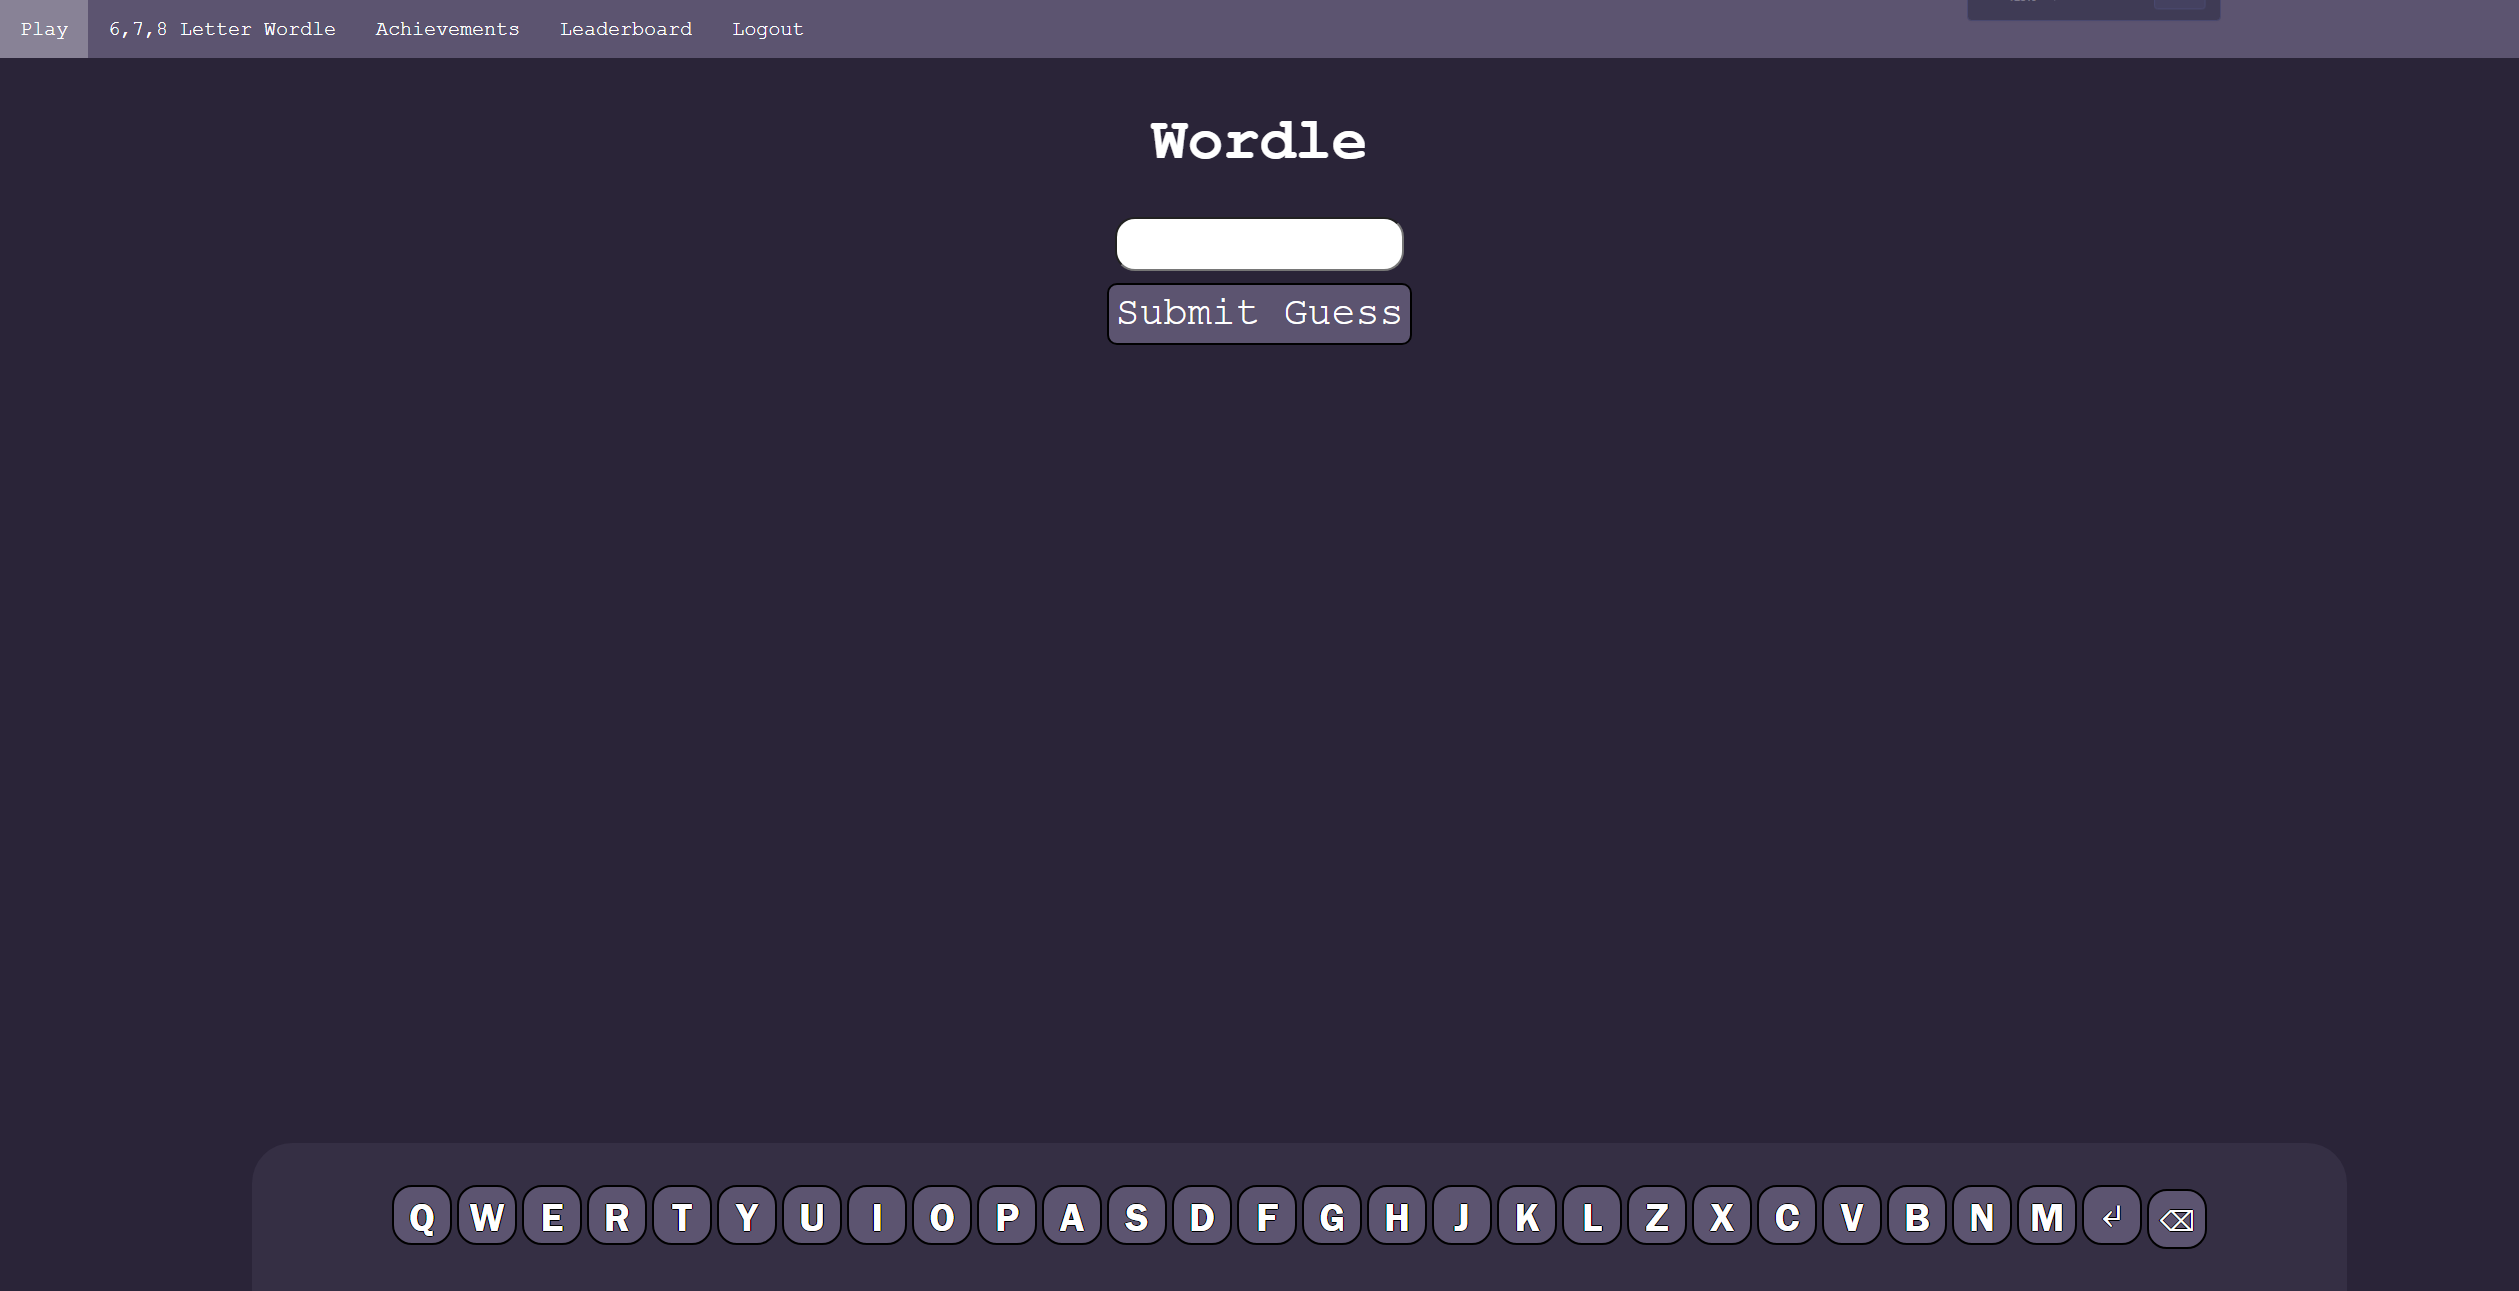
\includegraphics[width=\textwidth]{Picture_of_website.png} % Replace with your image file
    \label{fig:example}
    \end{figure}
    \vspace{1cm} % Adds some space between the text and the URLs

    \Large % Adjust the size as needed
    \texttt{\href{https://the-gauntlet-5a20b0d87ed3.herokuapp.com/wordle}{https://the-gauntlet-5a20b0d87ed3.herokuapp.com/wordle}} \\
    \vspace{0.5cm} % Adds some space between the two URLs
    \texttt{\href{https://wordle-no-login-c983e50c89bf.herokuapp.com}{https://wordle-no-login-c983e50c89bf.herokuapp.com}}
\end{center}